\documentclass[11pt,a4paper]{article}
\usepackage[utf8]{inputenc}
\usepackage[T1]{fontenc}
\usepackage{geometry}
\usepackage{hyperref}
\usepackage{listings}
\usepackage{xcolor}
\usepackage{graphicx}
\usepackage{amsmath}
\usepackage{parskip}
\usepackage{enumitem}
\usepackage{titlesec}
\usepackage{tikz}
\usetikzlibrary{shapes.geometric, arrows.meta, positioning, fit, calc}

\geometry{margin=1in}
\hypersetup{colorlinks=true, linkcolor=blue, urlcolor=blue}

% Code listing style
\definecolor{codegreen}{rgb}{0,0.6,0}
\definecolor{codegray}{rgb}{0.5,0.5,0.5}
\definecolor{codepurple}{rgb}{0.58,0,0.82}
\definecolor{backcolour}{rgb}{0.95,0.95,0.92}

\lstdefinestyle{mystyle}{
    backgroundcolor=\color{backcolour},
    commentstyle=\color{codegreen},
    keywordstyle=\color{codepurple}\bfseries,
    numberstyle=\tiny\color{codegray},
    stringstyle=\color{orange},
    basicstyle=\ttfamily\footnotesize,
    breakatwhitespace=false,
    breaklines=true,
    captionpos=b,
    keepspaces=true,
    numbers=left,
    numbersep=5pt,
    showspaces=false,
    showstringspaces=false,
    showtabs=false,
    tabsize=2
}

\lstset{style=mystyle}

\title{\textbf{RimRun: Technical Documentation} \\ \large A Basketball Court Discovery Mobile Application}
\author{RimRun Development Team}
\date{\today}

\begin{document}

\maketitle
\tableofcontents
\newpage

%==============================================================================
\section{Project Overview}
%==============================================================================

RimRun is a React Native mobile application built with Expo that helps users discover and share basketball courts. The application enables users to create accounts, complete their profiles with avatars and date of birth, and (in future phases) view courts on a map, add new courts, rate them, and engage in real-time community features.

\subsection*{How to Use This Document}

This document is written as a \textbf{learning guide}. Assume you did not build this project---you are learning from the developer. Each section explains \textit{what} a concept is, \textit{why} it is used, and \textit{how} it works in RimRun. We start with foundational concepts (like React Context) before diving into implementation details. Read sections in order for the best understanding.

\textbf{Current Implementation Status (Phase 1 MVP):}
\begin{itemize}
    \item User authentication (signup, login, sign out)
    \item Onboarding flow with optional profile picture and date of birth
    \item Profile tab with avatar display and update capability
    \item Username uniqueness validation
    \item Supabase backend for auth, database, and storage
\end{itemize}

%==============================================================================
\section{Tech Stack}
%==============================================================================

\begin{figure}[h]
\centering
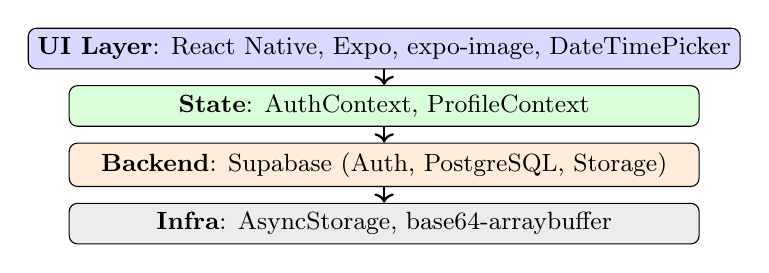
\begin{tikzpicture}[
  layer/.style={rectangle, draw, rounded corners=3pt, minimum width=8cm, minimum height=0.5cm, align=center, font=\small}
]
  \node[layer, fill=blue!15] (ui) {\textbf{UI Layer}: React Native, Expo, expo-image, DateTimePicker};
  \node[layer, fill=green!15, below=0.2cm of ui] (state) {\textbf{State}: AuthContext, ProfileContext};
  \node[layer, fill=orange!15, below=0.2cm of state] (backend) {\textbf{Backend}: Supabase (Auth, PostgreSQL, Storage)};
  \node[layer, fill=gray!15, below=0.2cm of backend] (infra) {\textbf{Infra}: AsyncStorage, base64-arraybuffer};
  \draw[->, thick] (ui) -- (state);
  \draw[->, thick] (state) -- (backend);
  \draw[->, thick] (backend) -- (infra);
\end{tikzpicture}
\caption{RimRun technology stack layers}
\end{figure}

\subsection{Core Framework}
\begin{itemize}
    \item \textbf{React Native 0.81.5} -- Cross-platform mobile development
    \item \textbf{Expo SDK 54} -- Development toolchain and native APIs
    \item \textbf{TypeScript 5.9} -- Type-safe JavaScript
    \item \textbf{Expo Router 6.0} -- File-based routing for React Native
\end{itemize}

\subsection{Backend \& Data}
\begin{itemize}
    \item \textbf{Supabase} -- Backend-as-a-Service (Auth, PostgreSQL, Storage, RLS)
    \item \textbf{AsyncStorage} -- Persistent session storage for Supabase auth tokens
\end{itemize}

\subsection{UI \& Media}
\begin{itemize}
    \item \textbf{expo-image} -- Optimized image component
    \item \textbf{expo-image-picker} -- Camera and photo library
    \item \textbf{@react-native-community/datetimepicker} -- Native date picker
    \item \textbf{react-native-safe-area-context} -- Safe area handling
\end{itemize}

\subsection{Why This Tech Stack Is Appropriate}

Each technology was chosen for a specific reason. Understanding the rationale helps you evaluate trade-offs and future improvements.

\begin{itemize}[leftmargin=*]
    \item \textbf{React Native + Expo}: React Native lets you build iOS and Android apps with one codebase using JavaScript/TypeScript. Expo adds a managed workflow: pre-built native modules (camera, storage, etc.), OTA updates, and simpler builds. For a small team or solo developer, this dramatically reduces the cost of supporting two platforms. The alternative---writing separate Swift/Kotlin apps---would double development time.
    
    \item \textbf{Supabase}: Supabase is a Backend-as-a-Service (BaaS). It provides authentication, a PostgreSQL database, and file storage out of the box. You do not need to run your own servers or write backend API code. For an MVP, this is ideal: you focus on the app, not infrastructure. Supabase also uses Row Level Security (RLS), so you can enforce ``users only see their own data'' directly in the database.
    
    \item \textbf{AsyncStorage}: React Native does not have \texttt{localStorage} like web browsers. AsyncStorage is the mobile equivalent: a simple key-value store that persists data across app restarts. Supabase needs this to store auth tokens so users stay logged in after closing the app.
    
    \item \textbf{TypeScript}: TypeScript adds static types to JavaScript. It catches many bugs at compile time (e.g., typos in property names, wrong argument types) and improves editor autocomplete. For a project that will grow, the upfront cost of typing pays off in fewer runtime errors.
\end{itemize}

\subsection{Possible Improvements}

\begin{itemize}[leftmargin=*]
    \item \textbf{State management}: For larger apps, consider Zustand or Redux Toolkit instead of (or in addition to) Context. Context causes all consumers to re-render when the value changes; for fine-grained updates, a store-based solution can be more efficient.
    
    \item \textbf{Offline support}: Supabase does not cache data by default. Adding offline-first logic (e.g., with Supabase's real-time subscriptions plus local SQLite) would improve UX when the network is poor.
    
    \item \textbf{Testing}: Add unit tests (Jest) for contexts and utilities, and E2E tests (Detox or Maestro) for critical flows like sign-up and profile update.
    
    \item \textbf{Error boundaries}: Wrap route groups in React Error Boundaries to catch crashes and show a fallback UI instead of a blank screen.
    
    \item \textbf{Image optimization}: Consider resizing/compressing images before upload to reduce storage costs and load times. The current implementation uploads full-quality images.
\end{itemize}

%==============================================================================
\section{Understanding React Context}
%==============================================================================

Before we discuss AuthContext and ProfileContext, you need to understand \textbf{React Context}. This is a core React feature that RimRun relies on heavily.

\subsection{What Is Context?}

In React, data flows \textit{down} from parent to child via \textbf{props}. A parent component passes data to its children, and those children pass it to their children, and so on. This works well for simple trees.

The problem: sometimes many components need the same data (e.g., the current user). Passing that data through every level of the tree is tedious and error-prone. This is called \textbf{prop drilling}.

\subsection{The Prop Drilling Problem}

Imagine: \texttt{App} has the current user. \texttt{App} renders \texttt{Layout}, which renders \texttt{ProfileTab}, which renders \texttt{Avatar}. The \texttt{Avatar} needs the user's ID to load their picture. Without Context, you would have to pass \texttt{user} from \texttt{App} $\rightarrow$ \texttt{Layout} $\rightarrow$ \texttt{ProfileTab} $\rightarrow$ \texttt{Avatar}. Every intermediate component must accept and forward \texttt{user} even if it does not use it. If you add a new screen that also needs the user, you must thread the prop through again.

\subsection{How Context Solves It}

\textbf{Context} lets you create a ``channel'' that any descendant component can subscribe to, without passing props through every level. You wrap part of your tree in a \textbf{Provider} that holds the value. Any child (no matter how deep) can call \texttt{useContext(MyContext)} to read that value directly.

\begin{lstlisting}[language=TypeScript, caption=Conceptual Context Usage]
// 1. Create a context
const UserContext = createContext<User | null>(null);

// 2. Provide a value at the top
function App() {
  const [user, setUser] = useState<User | null>(null);
  return (
    <UserContext.Provider value={user}>
      <Layout />  {/* Layout doesn't need to know about user */}
    </UserContext.Provider>
  );
}

// 3. Consume anywhere deep in the tree
function Avatar() {
  const user = useContext(UserContext);  // Direct access!
  return <Image source={{ uri: user?.avatarUrl }} />;
}
\end{lstlisting}

\subsection{Why RimRun Uses Context}

RimRun uses Context for two main pieces of app-wide state:

\begin{enumerate}
    \item \textbf{AuthContext}: Who is logged in (user, session). Needed by login screens, the profile tab, and future features like ``add a court'' (you must be logged in).
    \item \textbf{ProfileContext}: The user's profile data (username, avatar URL, date of birth). Needed by the profile tab and onboarding.
\end{enumerate}

Without Context, every screen would need to receive \texttt{user} and \texttt{profile} as props from a common ancestor. With Context, any component can call \texttt{useAuth()} or \texttt{useProfile()} and get the data it needs. The architecture stays clean and scalable.

%==============================================================================
\section{Application Architecture}
%==============================================================================

\subsection{Provider Hierarchy}

\begin{figure}[h]
\centering
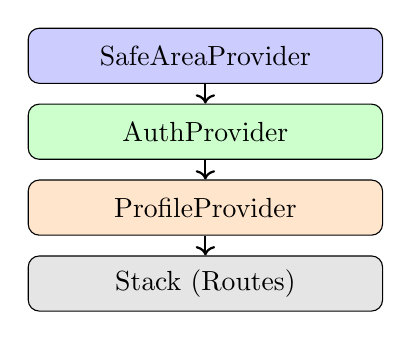
\begin{tikzpicture}[
  box/.style={rectangle, draw, rounded corners=4pt, minimum width=4.5cm, minimum height=0.7cm, align=center},
  arrow/.style={->, thick}
]
  \node[box, fill=blue!20] (safe) {SafeAreaProvider};
  \node[box, fill=green!20, below=0.25cm of safe] (auth) {AuthProvider};
  \node[box, fill=orange!20, below=0.25cm of auth] (profile) {ProfileProvider};
  \node[box, fill=gray!20, below=0.25cm of profile] (stack) {Stack (Routes)};
  \draw[arrow] (safe.south) -- (auth.north);
  \draw[arrow] (auth.south) -- (profile.north);
  \draw[arrow] (profile.south) -- (stack.north);
\end{tikzpicture}
\caption{Provider nesting: outer providers wrap inner. ProfileProvider depends on AuthProvider (uses \texttt{useAuth}).}
\end{figure}

The application uses a nested provider structure in \texttt{app/\_layout.tsx}. \textbf{Order matters}: AuthProvider must wrap ProfileProvider because ProfileContext calls \texttt{useAuth()}. A hook can only be used within a component that is a descendant of the corresponding Provider. Since ProfileProvider uses \texttt{useAuth()}, it must be rendered inside AuthProvider. SafeAreaProvider is outermost so all screens can use safe area insets (e.g., for notches).

\subsection{Screen Flow}

\begin{figure}[h]
\centering
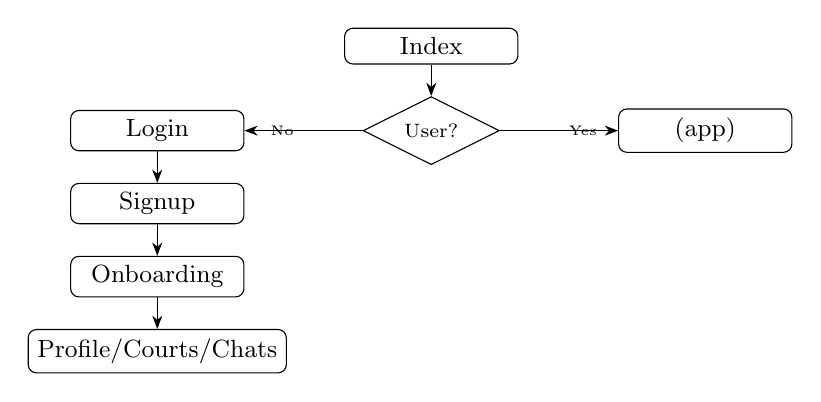
\begin{tikzpicture}[
  node/.style={rectangle, draw, rounded corners=3pt, minimum width=2.2cm, align=center, font=\small},
  decision/.style={diamond, draw, aspect=2, minimum width=1.5cm, align=center, font=\scriptsize},
  arrow/.style={->, >=Stealth}
]
  \node[node] (index) {Index};
  \node[decision, below=0.4cm of index] (auth) {User?};
  \node[node, left=1.5cm of auth] (login) {Login};
  \node[node, right=1.5cm of auth] (app) {(app)};
  \node[node, below=0.4cm of login] (signup) {Signup};
  \node[node, below=0.4cm of signup] (onboard) {Onboarding};
  \node[node, below=0.4cm of onboard] (tabs) {Profile/Courts/Chats};

  \draw[arrow] (index) -- (auth);
  \draw[arrow] (auth) -- node[left, font=\tiny] {No} (login);
  \draw[arrow] (auth) -- node[right, font=\tiny] {Yes} (app);
  \draw[arrow] (login) -- (signup);
  \draw[arrow] (signup) -- (onboard);
  \draw[arrow] (onboard) -- (tabs);
\end{tikzpicture}
\caption{Application navigation flow}
\end{figure}

\subsection{Route Structure}

Expo Router uses \textbf{file-based routing}: the folder structure under \texttt{app/} defines the routes.

\begin{itemize}[leftmargin=*]
    \item \texttt{/} -- Index. Typically redirects to login (if not authenticated) or to \texttt{/(app)} (if authenticated).
    \item \texttt{/(auth)/login}, \texttt{signup}, \texttt{onboarding}, \texttt{reset-password} -- Auth flow screens. Parentheses in \texttt{(auth)} mean it is a \textit{route group}: it groups files without adding a segment to the URL (so \texttt{/(auth)/login} is just \texttt{/login}).
    \item \texttt{/(app)} -- Main app with tabs (profile, courts, chats). Shown only after the user is authenticated and has completed onboarding.
\end{itemize}

\subsection{How the App Decides What to Show}

The index route and layout components use \texttt{useAuth()} to read \texttt{user} and \texttt{loading}. If \texttt{loading} is true, a loading screen is shown. If \texttt{user} is null, the user is redirected to login/signup. If \texttt{user} exists but the profile is incomplete (e.g., no date of birth), the user may be sent to onboarding. Once everything is ready, the user sees the main \texttt{/(app)} tabs.

%==============================================================================
\section{Supabase Client Configuration}
%==============================================================================

The Supabase client is the bridge between your app and Supabase's services (Auth, Database, Storage). It is created once and reused everywhere.

\subsection{Why \texttt{AsyncStorage} for Auth?}

On the web, Supabase uses \texttt{localStorage} to persist the session (tokens) so users stay logged in after refreshing. React Native does not have \texttt{localStorage}. \textbf{AsyncStorage} is the React Native equivalent: a simple key-value store that survives app restarts. By passing \texttt{AsyncStorage} to the Supabase client's \texttt{auth.storage} option, we tell Supabase: ``Store session tokens here.'' Without this, every app restart would log the user out.

\subsection{Other Auth Options Explained}

\begin{itemize}[leftmargin=*]
    \item \textbf{autoRefreshToken: true}: JWTs expire. Supabase can automatically refresh them before expiry so the user does not get logged out mid-session.
    \item \textbf{persistSession: true}: Save the session to storage (AsyncStorage) so it survives app restarts.
    \item \textbf{detectSessionInUrl: false}: On the web, Supabase can detect magic links or OAuth callbacks from the URL. Mobile apps typically do not use URL-based auth, so this is disabled.
\end{itemize}

\subsection{Main Supabase Client (\texttt{lib/supabase.ts})}

\begin{lstlisting}[language=TypeScript, caption=Supabase Client Configuration]
export const supabase = createClient(supabaseUrl, supabaseAnonKey, {
  auth: {
    storage: AsyncStorage,      // Persist session (no localStorage in RN)
    autoRefreshToken: true,     // Refresh JWT before expiry
    persistSession: true,       // Keep user logged in
    detectSessionInUrl: false,  // Not needed for mobile
  }
})
\end{lstlisting}

\begin{figure}[h]
\centering
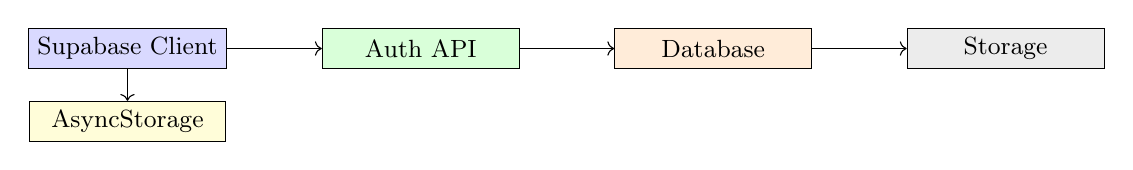
\begin{tikzpicture}[
  box/.style={rectangle, draw, minimum width=2.5cm, minimum height=0.5cm, align=center, font=\small}
]
  \node[box, fill=blue!15] (client) {Supabase Client};
  \node[box, fill=green!15, right=1.2cm of client] (auth) {Auth API};
  \node[box, fill=orange!15, right=1.2cm of auth] (db) {Database};
  \node[box, fill=gray!15, right=1.2cm of db] (storage) {Storage};
  \node[box, fill=yellow!15, below=0.4cm of client] (async) {AsyncStorage};
  \draw[->] (client) -- (auth);
  \draw[->] (auth) -- (db);
  \draw[->] (db) -- (storage);
  \draw[->] (client) -- (async);
\end{tikzpicture}
\caption{Supabase client components and session persistence}
\end{figure}

%==============================================================================
\section{AuthContext}
%==============================================================================

\subsection{What AuthContext Does}

AuthContext is a React Context that manages \textbf{authentication state}---who is logged in---and provides auth actions (sign in, sign up, sign out). Think of it as the ``single source of truth'' for whether a user is authenticated and who they are.

\subsection{Why Auth Is Separate From Profile}

You might wonder: why not put both user and profile in one context? The answer is \textbf{separation of concerns} and \textbf{dependency order}.

\begin{itemize}[leftmargin=*]
    \item \textbf{Auth} answers: ``Is someone logged in? Who?'' It comes from Supabase Auth and is available as soon as the session is restored (or after sign-in).
    \item \textbf{Profile} answers: ``What is this user's username, avatar, date of birth?'' It comes from the \texttt{profiles} table and depends on \texttt{user.id}. You cannot fetch a profile without knowing the user's ID first.
\end{itemize}

By keeping them separate, AuthContext can initialize and restore the session independently. ProfileContext then uses \texttt{useAuth()} to get \texttt{user.id} and fetch the profile. If we combined them, we would have circular dependencies and harder-to-reason-about initialization. Also, auth state changes (e.g., sign out) are distinct from profile updates; separating them keeps the logic clean.

\subsection{How AuthContext Works: Step by Step}

\subsubsection{1. Initialization and Session Restoration}

When the app starts, the user might already be logged in (from a previous session). Supabase stores the session in AsyncStorage. AuthContext must:

\begin{enumerate}
    \item Call \texttt{supabase.auth.getSession()} to read the stored session.
    \item If a session exists, set \texttt{user} and \texttt{session} in state so the rest of the app knows someone is logged in.
    \item Set \texttt{loading} to \texttt{false} when done (or after a timeout) so the app can show the correct screen (login vs. main app).
\end{enumerate}

\subsubsection{2. The \texttt{onAuthStateChange} Listener}

Supabase fires \texttt{onAuthStateChange} whenever auth state changes: sign in, sign out, token refresh, etc. AuthContext subscribes to this listener and updates \texttt{user} and \texttt{session} whenever it fires. That way, you never have to manually call \texttt{setUser} after \texttt{signIn} or \texttt{signOut}---the listener does it for you. This keeps the auth state in sync with Supabase.

\subsubsection{3. The \texttt{loading} State}

Until \texttt{getSession()} completes, we do not know if the user is logged in. During this time, \texttt{loading} is \texttt{true}. The app typically shows a loading screen. There is also a 5-second timeout: if \texttt{getSession} hangs (e.g., network issues), we still set \texttt{loading} to \texttt{false} so the user is not stuck.

\subsubsection{4. Sign-In with Username or Email}

Supabase Auth uses \textbf{email + password}. RimRun allows users to sign in with either their email or their username. If the input contains \texttt{@}, we treat it as an email. Otherwise, we query the \texttt{profiles} table for a row whose \texttt{username} matches (case-insensitive), get the \texttt{email}, and use that for \texttt{signInWithPassword}. This gives users flexibility without changing how Supabase Auth works.

\subsubsection{5. Sign-Up with Username in Metadata}

Supabase \texttt{signUp} accepts \texttt{options.data}, which is stored as \textbf{user metadata}. RimRun passes \texttt{username} there. A database trigger (or Edge Function) can then create a row in \texttt{profiles} with that username when the user is created. The AuthContext does not create the profile row itself---that is handled by the backend.

\subsection{Auth State Flow}

\begin{figure}[h]
\centering
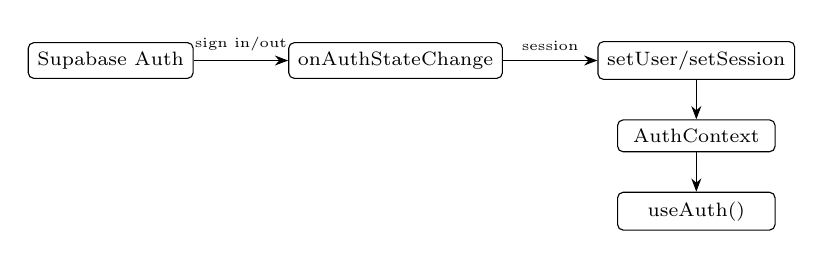
\begin{tikzpicture}[
  node/.style={rectangle, draw, rounded corners=2pt, minimum width=2cm, align=center, font=\scriptsize},
  arrow/.style={->, >=Stealth}
]
  \node[node] (supabase) {Supabase Auth};
  \node[node, right=1.2cm of supabase] (listener) {onAuthStateChange};
  \node[node, right=1.2cm of listener] (state) {setUser/setSession};
  \node[node, below=0.5cm of state] (context) {AuthContext};
  \node[node, below=0.5cm of context] (components) {useAuth()};

  \draw[arrow] (supabase) -- node[above, font=\tiny] {sign in/out} (listener);
  \draw[arrow] (listener) -- node[above, font=\tiny] {session} (state);
  \draw[arrow] (state) -- (context);
  \draw[arrow] (context) -- (components);
\end{tikzpicture}
\caption{Auth state propagation from Supabase to components}
\end{figure}

\subsection{Sign-In with Username or Email}

\begin{figure}[h]
\centering
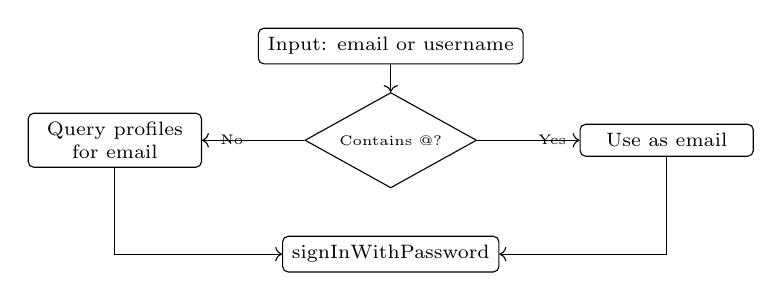
\begin{tikzpicture}[
  node/.style={rectangle, draw, rounded corners=2pt, minimum width=2.2cm, align=center, font=\scriptsize},
  decision/.style={diamond, draw, aspect=1.8, minimum width=1.2cm, align=center, font=\tiny}
]
  \node[node] (input) {Input: email or username};
  \node[decision, below=0.35cm of input] (check) {Contains @?};
  \node[node, left=1.3cm of check] (query) {Query profiles\\for email};
  \node[node, right=1.3cm of check] (use) {Use as email};
  \node[node, below=0.6cm of check] (signin) {signInWithPassword};

  \draw[->] (input) -- (check);
  \draw[->] (check) -- node[left, font=\tiny] {No} (query);
  \draw[->] (check) -- node[right, font=\tiny] {Yes} (use);
  \draw[->] (query) |- (signin);
  \draw[->] (use) |- (signin);
\end{tikzpicture}
\caption{Username-to-email resolution for sign-in}
\end{figure}

\subsection{Sign-Up with User Metadata}

\begin{lstlisting}[language=TypeScript, caption=Sign-Up with Username in Metadata]
await supabase.auth.signUp({
  email, password,
  options: { data: { username } },  // For profile trigger
});
\end{lstlisting}

%==============================================================================
\section{ProfileContext}
%==============================================================================

\subsection{What ProfileContext Does}

ProfileContext manages \textbf{profile data}---username, avatar URL, date of birth---from the \texttt{profiles} table. It also provides \texttt{updateProfilePicture}, which lets the user pick an image (camera or library), upload it to Supabase Storage, and update the profile with the new URL.

\subsection{Why ProfileContext Depends on AuthContext}

ProfileContext calls \texttt{useAuth()} to get \texttt{user}. It needs \texttt{user.id} to:

\begin{enumerate}
    \item \textbf{Fetch the profile}: The \texttt{profiles} table has a row per user, keyed by \texttt{id} (which matches \texttt{auth.users.id}). We query \texttt{profiles} where \texttt{id = user.id}.
    \item \textbf{Upload avatars}: Supabase Storage paths use \texttt{\{user\_id\}/avatar.jpg}. We need \texttt{user.id} to construct the path and to satisfy RLS (users can only write to their own folder).
\end{enumerate}

Because ProfileContext uses \texttt{useAuth()}, it must be rendered \textit{inside} AuthProvider. That is why the provider order in \texttt{\_layout.tsx} is: SafeAreaProvider $\rightarrow$ AuthProvider $\rightarrow$ ProfileProvider.

\subsection{How ProfileContext Works: Step by Step}

\subsubsection{1. Fetching the Profile}

When \texttt{user} changes (e.g., user logs in), \texttt{fetchProfile} runs. It queries \texttt{profiles} for the row with \texttt{id = user.id}, selects \texttt{profile\_image\_url}, \texttt{date\_of\_birth}, \texttt{username}, and \texttt{email}, and stores the result in \texttt{profile} state. If \texttt{user} is null (signed out), \texttt{profile} is set to null.

\subsubsection{2. \texttt{refreshProfile}}

The context exposes \texttt{refreshProfile}, which is the same as \texttt{fetchProfile}. Screens can call it to reload profile data after an update (e.g., after onboarding saves the date of birth).

\subsubsection{3. \texttt{updateProfilePicture}}

When the user taps to change their avatar, \texttt{updateProfilePicture} shows an \texttt{Alert.alert} with options: Camera or Photo Library. Based on the choice, it requests the appropriate permission, launches the image picker, and receives a base64 string. It then:

\begin{enumerate}
    \item Decodes base64 to an ArrayBuffer (Supabase Storage expects binary data).
    \item Uploads to \texttt{avatars/\{user.id\}/avatar.jpg} with \texttt{upsert: true} (overwrites if exists).
    \item Gets the public URL for the uploaded file.
    \item Updates the \texttt{profiles} row with the new \texttt{profile\_image\_url}.
    \item Updates local \texttt{profile} state so the UI reflects the change immediately.
\end{enumerate}

If the user cancels the picker or permission is denied, nothing is uploaded. On upload error, an alert is shown.

\subsection{Profile Data Flow}

\begin{figure}[h]
\centering
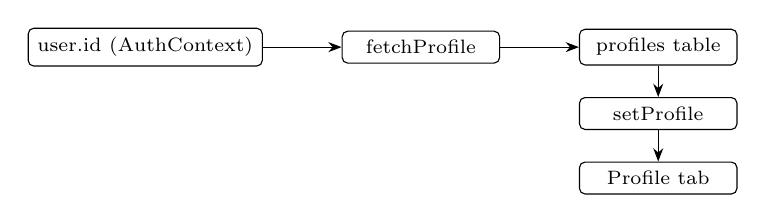
\begin{tikzpicture}[
  node/.style={rectangle, draw, rounded corners=2pt, minimum width=2cm, align=center, font=\scriptsize},
  arrow/.style={->, >=Stealth}
]
  \node[node] (user) {user.id (AuthContext)};
  \node[node, right=1cm of user] (fetch) {fetchProfile};
  \node[node, right=1cm of fetch] (supabase) {profiles table};
  \node[node, below=0.4cm of supabase] (state) {setProfile};
  \node[node, below=0.4cm of state] (ui) {Profile tab};

  \draw[arrow] (user) -- (fetch);
  \draw[arrow] (fetch) -- (supabase);
  \draw[arrow] (supabase) -- (state);
  \draw[arrow] (state) -- (ui);
\end{tikzpicture}
\caption{Profile fetch flow: user.id triggers fetch, data flows to UI}
\end{figure}

%==============================================================================
\section{Expo Image Picker}
%==============================================================================

\subsection{What the Image Picker Does}

\textbf{expo-image-picker} lets users select an image from their photo library or take a new photo with the camera. RimRun uses it for profile pictures. On tap, the app shows an alert: ``Camera'' or ``Photo Library.'' The user picks one, and the picker returns the selected image (or null if canceled).

\subsection{Why \texttt{base64: true}?}

Supabase Storage's \texttt{upload} method expects binary data (e.g., \texttt{ArrayBuffer} or \texttt{Blob}). On the web, \texttt{File} and \texttt{Blob} work well. In React Native, these APIs are not fully reliable with Supabase. The recommended approach is to get the image as a \textbf{base64} string from the picker, then use \texttt{decode()} from \texttt{base64-arraybuffer} to convert it to an \texttt{ArrayBuffer} before uploading. That is why \texttt{base64: true} is set in the picker options.

\subsection{Source Selection Flow}

\begin{figure}[h]
\centering
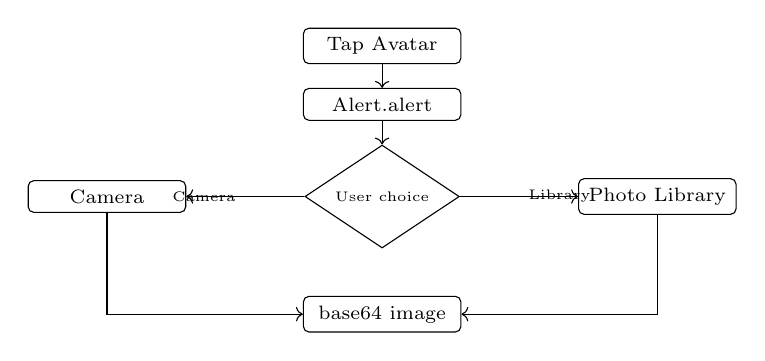
\begin{tikzpicture}[
  node/.style={rectangle, draw, rounded corners=2pt, minimum width=2cm, align=center, font=\scriptsize},
  decision/.style={diamond, draw, aspect=1.5, minimum width=1.4cm, align=center, font=\tiny}
]
  \node[node] (tap) {Tap Avatar};
  \node[node, below=0.3cm of tap] (alert) {Alert.alert};
  \node[decision, below=0.3cm of alert] (choice) {User choice};
  \node[node, left=1.5cm of choice] (camera) {Camera};
  \node[node, right=1.5cm of choice] (library) {Photo Library};
  \node[node, below=0.6cm of choice] (result) {base64 image};

  \draw[->] (tap) -- (alert);
  \draw[->] (alert) -- (choice);
  \draw[->] (choice) -- node[left, font=\tiny] {Camera} (camera);
  \draw[->] (choice) -- node[right, font=\tiny] {Library} (library);
  \draw[->] (camera) |- (result);
  \draw[->] (library) |- (result);
\end{tikzpicture}
\caption{Image picker flow: Alert presents options, then Camera or Library returns base64}
\end{figure}

\subsection{Picker Options Explained}

\begin{lstlisting}[language=TypeScript, caption=Image Picker Configuration]
const options = {
  mediaTypes: ['images'],
  allowsEditing: true,   // Crop to square
  aspect: [1, 1],
  quality: 1,
  base64: true,         // Required for Supabase
};
\end{lstlisting}

\begin{itemize}[leftmargin=*]
    \item \textbf{mediaTypes: ['images']}: Only allow images (no video).
    \item \textbf{allowsEditing: true}: After selection, show a crop UI. This lets users crop to a square, which looks better for avatars.
    \item \textbf{aspect: [1, 1]}: Enforce a 1:1 (square) aspect ratio for the crop.
    \item \textbf{quality: 1}: Full quality (0--1 scale). Lower values reduce file size but may look worse.
    \item \textbf{base64: true}: Return the image as a base64 string so we can decode and upload to Supabase.
\end{itemize}

%==============================================================================
\section{DateTimePicker}
%==============================================================================

\subsection{What the DateTimePicker Does}

The \textbf{@react-native-community/datetimepicker} component shows a native date picker. On iOS, it appears as a wheel; on Android, as a calendar dialog. RimRun uses it in onboarding for the user's date of birth.

\subsection{Why Platform-Specific Handling?}

iOS and Android render the picker differently and fire events differently. On Android, when the user dismisses the dialog without selecting a date, \texttt{onChange} is still called with \texttt{event.type === 'dismissed'}. If we updated state in that case, we would overwrite the user's previous selection with \texttt{undefined}. So we only update state when \texttt{event.type === 'set'} (user confirmed a date). On iOS, the behavior is different, and \texttt{textColor} can be used to style the wheel.

\subsection{Platform Display Modes}

\begin{figure}[h]
\centering
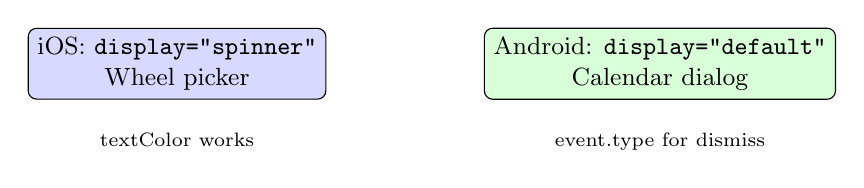
\begin{tikzpicture}[
  node/.style={rectangle, draw, rounded corners=3pt, minimum width=3cm, align=center, font=\small}
]
  \node[node, fill=blue!15] (ios) {iOS: \texttt{display="spinner"}\\Wheel picker};
  \node[node, fill=green!15, right=2cm of ios] (android) {Android: \texttt{display="default"}\\Calendar dialog};
  \node[below=0.3cm of ios, font=\scriptsize] {textColor works};
  \node[below=0.3cm of android, font=\scriptsize] {event.type for dismiss};
\end{tikzpicture}
\caption{Platform-specific DateTimePicker behavior}
\end{figure}

\subsection{Event Handling (Android)}

\begin{figure}[h]
\centering
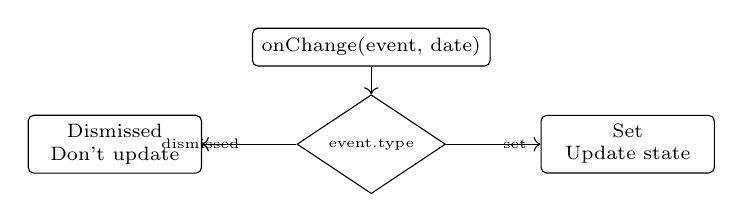
\begin{tikzpicture}[
  node/.style={rectangle, draw, rounded corners=2pt, minimum width=2.2cm, align=center, font=\scriptsize},
  decision/.style={diamond, draw, aspect=1.5, minimum width=1.2cm, align=center, font=\tiny}
]
  \node[node] (onchange) {onChange(event, date)};
  \node[decision, below=0.35cm of onchange] (type) {event.type};
  \node[node, left=1.2cm of type] (dismiss) {Dismissed\\Don't update};
  \node[node, right=1.2cm of type] (set) {Set\\Update state};

  \draw[->] (onchange) -- (type);
  \draw[->] (type) -- node[left, font=\tiny] {dismissed} (dismiss);
  \draw[->] (type) -- node[right, font=\tiny] {set} (set);
\end{tikzpicture}
\caption{Android: Only update state when \texttt{event.type === 'set'}}
\end{figure}

%==============================================================================
\section{Profile Picture Upload Flow}
%==============================================================================

This section ties together Image Picker, Supabase Storage, and the \texttt{profiles} table. When a user selects or takes a photo, the app must: (1) get the image data, (2) upload it to Storage, (3) get a public URL, (4) save that URL in the \texttt{profiles} table, and (5) update the UI.

\subsection{End-to-End Pipeline}
\begin{figure}[h]
\centering
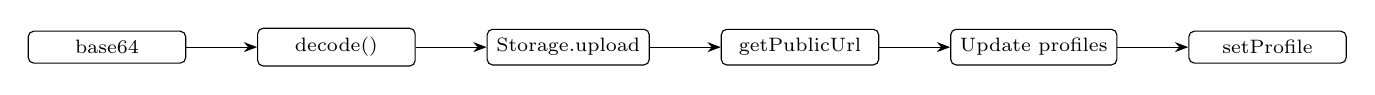
\begin{tikzpicture}[
  node/.style={rectangle, draw, rounded corners=2pt, minimum width=2cm, align=center, font=\scriptsize},
  arrow/.style={->, >=Stealth}
]
  \node[node] (1) {base64};
  \node[node, right=0.9cm of 1] (2) {decode()};
  \node[node, right=0.9cm of 2] (3) {Storage.upload};
  \node[node, right=0.9cm of 3] (4) {getPublicUrl};
  \node[node, right=0.9cm of 4] (5) {Update profiles};
  \node[node, right=0.9cm of 5] (6) {setProfile};

  \draw[arrow] (1) -- (2);
  \draw[arrow] (2) -- (3);
  \draw[arrow] (3) -- (4);
  \draw[arrow] (4) -- (5);
  \draw[arrow] (5) -- (6);
\end{tikzpicture}
\caption{End-to-end profile picture upload pipeline}
\end{figure}

\subsection{Why base64 and \texttt{decode()}?}

React Native does not support \texttt{Blob} and \texttt{File} APIs the same way browsers do. Supabase Storage's \texttt{upload()} expects binary data (e.g., \texttt{ArrayBuffer}). The flow is: ImagePicker returns base64 $\rightarrow$ \texttt{decode()} from \texttt{base64-arraybuffer} converts it to \texttt{ArrayBuffer} $\rightarrow$ \texttt{storage.upload()} sends it to Supabase. This is the recommended pattern for React Native + Supabase.

%==============================================================================
\section{Supabase Storage \& Buckets}
%==============================================================================

\subsection{What Is a Bucket?}

Supabase Storage organizes files in \textbf{buckets}---like folders at the top level. RimRun uses an \texttt{avatars} bucket for profile pictures. Each user gets a folder named by their \texttt{user.id}, and the avatar file is stored as \texttt{\{user\_id\}/avatar.jpg}. Using \texttt{upsert: true} on upload means a new picture overwrites the old one, so each user effectively has one avatar file.

\subsection{Bucket Structure}

\begin{figure}[h]
\centering
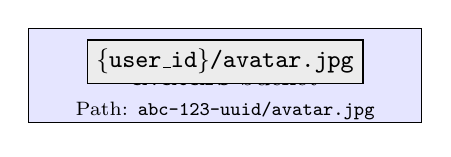
\begin{tikzpicture}[
  bucket/.style={rectangle, draw, minimum width=5cm, minimum height=1.2cm},
  file/.style={rectangle, draw, fill=gray!15, font=\ttfamily\small}
]
  \node[bucket, fill=blue!10] (avatars) {\textbf{avatars} bucket};
  \node[file, below=0.15cm of avatars.north, anchor=north] (f1) {\{user\_id\}/avatar.jpg};
  \node[below=0.1cm of f1, font=\scriptsize] {Path: \texttt{abc-123-uuid/avatar.jpg}};
\end{tikzpicture}
\caption{Avatars bucket: one file per user, overwritten with \texttt{upsert: true}}
\end{figure}

\subsection{Storage Policies (RLS)}

\begin{figure}[h]
\centering
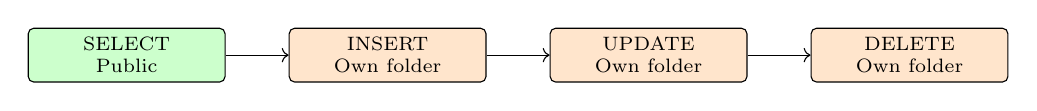
\begin{tikzpicture}[
  policy/.style={rectangle, draw, rounded corners=2pt, minimum width=2.5cm, align=center, font=\scriptsize}
]
  \node[policy, fill=green!20] (sel) {SELECT\\Public};
  \node[policy, fill=orange!20, right=0.8cm of sel] (ins) {INSERT\\Own folder};
  \node[policy, fill=orange!20, right=0.8cm of ins] (upd) {UPDATE\\Own folder};
  \node[policy, fill=orange!20, right=0.8cm of upd] (del) {DELETE\\Own folder};

  \draw[->] (sel) -- (ins);
  \draw[->] (ins) -- (upd);
  \draw[->] (upd) -- (del);
\end{tikzpicture}
\caption{Storage policies: public read; authenticated users can only modify their own folder}
\end{figure}

\begin{itemize}[leftmargin=*]
    \item \textbf{SELECT (read)}: Public. Anyone can view avatar URLs (they are used in \texttt{profile\_image\_url} and displayed in the app).
    \item \textbf{INSERT, UPDATE, DELETE}: Only the authenticated user can modify files in their own folder. The path rule \texttt{(storage.foldername(name))[1] = auth.uid()::text} extracts the first folder from the path (e.g., \texttt{abc-123-uuid} from \texttt{abc-123-uuid/avatar.jpg}) and checks it equals the current user's ID. This prevents User A from overwriting User B's avatar.
\end{itemize}

%==============================================================================
\section{Database Schema}
%==============================================================================

\subsection{How Auth and Profiles Relate}

Supabase Auth manages \texttt{auth.users}: email, password hash, and metadata. When a user signs up, a row is created there. RimRun also has a \texttt{profiles} table with app-specific data: username, profile\_image\_url, date\_of\_birth. Each profile row has an \texttt{id} that matches \texttt{auth.users.id} (a foreign key). A database trigger typically creates a profile row when a user signs up, using the \texttt{username} from sign-up metadata.

\subsection{profiles Table \& Relationships}

\begin{figure}[h]
\centering
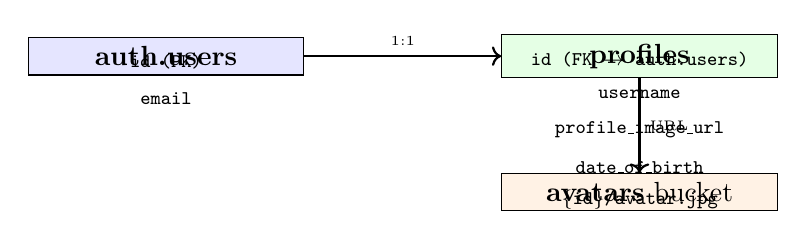
\begin{tikzpicture}[
  table/.style={rectangle, draw, minimum width=3.5cm},
  col/.style={font=\ttfamily\scriptsize}
]
  \node[table, fill=blue!10] (auth) {\textbf{auth.users}};
  \node[col, below=0.1cm of auth.north, anchor=north] (authid) {id (PK)};
  \node[col, below=0.05cm of authid] (authemail) {email};

  \node[table, fill=green!10, right=2.5cm of auth] (prof) {\textbf{profiles}};
  \node[col, below=0.1cm of prof.north, anchor=north] (profid) {id (FK $\rightarrow$ auth.users)};
  \node[col, below=0.05cm of profid] (profuser) {username};
  \node[col, below=0.05cm of profuser] (profimg) {profile\_image\_url};
  \node[col, below=0.05cm of profimg] (profdob) {date\_of\_birth};

  \node[table, fill=orange!10, below=1.2cm of prof] (storage) {\textbf{avatars} bucket};
  \node[col, below=0.1cm of storage.north, anchor=north] (path) {\{id\}/avatar.jpg};

  \draw[->, thick] (auth) -- node[above, font=\tiny] {1:1} (prof);
  \draw[->, thick] (prof) -- node[right, font=\tiny] {URL} (storage);
\end{tikzpicture}
\caption{Database relationships: auth.users $\rightarrow$ profiles $\rightarrow$ storage URL}
\end{figure}

%==============================================================================
\section{Storage Module (\texttt{lib/supabase/storage.ts})}
%==============================================================================

The project includes an alternative upload helper using \texttt{expo-file-system}'s \texttt{File} API. The \textbf{primary implementation} (onboarding, ProfileContext) uses the base64 + \texttt{decode()} approach, which is the recommended pattern for React Native with Supabase. The File API alternative exists for cases where you might want to upload from a file path instead of in-memory base64; for profile pictures chosen via ImagePicker, base64 is simpler and works reliably.

%==============================================================================
\section{Theme \& Constants}
%==============================================================================

RimRun centralizes design tokens in \texttt{constants/theme.ts}. Using shared \texttt{colors}, \texttt{spacing}, and \texttt{borderRadius} keeps the UI consistent and makes it easy to change the look globally (e.g., switch to a different primary color). Components import these constants instead of hardcoding values.

\begin{lstlisting}[language=TypeScript, caption=Theme Constants]
export const colors = {
  primary: '#E85D04', background: '#0F1419',
  surface: '#1A1F26', text: '#FFFFFF',
  textSecondary: '#94A3B8', error: '#EF4444',
};
export const spacing = { xs: 4, sm: 8, md: 16, lg: 24, xl: 32 };
export const borderRadius = { sm: 8, md: 12, lg: 16, full: 9999 };
\end{lstlisting}

%==============================================================================
\section{Summary}
%==============================================================================

\begin{figure}[h]
\centering
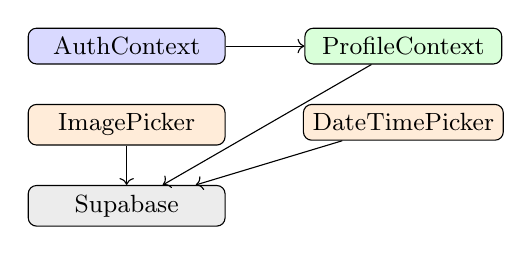
\begin{tikzpicture}[
  box/.style={rectangle, draw, rounded corners=3pt, minimum width=2.5cm, align=center, font=\small}
]
  \node[box, fill=blue!15] (auth) {AuthContext};
  \node[box, fill=green!15, right=1cm of auth] (profile) {ProfileContext};
  \node[box, fill=orange!15, below=0.5cm of auth] (picker) {ImagePicker};
  \node[box, fill=orange!15, below=0.5cm of profile] (date) {DateTimePicker};
  \node[box, fill=gray!15, below=0.5cm of picker] (supabase) {Supabase};

  \draw[->] (auth) -- (profile);
  \draw[->] (picker) -- (supabase);
  \draw[->] (date) -- (supabase);
  \draw[->] (profile) -- (supabase);
\end{tikzpicture}
\caption{Phase 1 MVP component overview}
\end{figure}

\subsection{Key Takeaways}

\begin{enumerate}
    \item \textbf{Context} solves prop drilling by letting any descendant access shared state via \texttt{useContext}. AuthContext and ProfileContext provide app-wide auth and profile data.
    \item \textbf{AuthContext} is the source of truth for who is logged in. It uses \texttt{onAuthStateChange} to stay in sync with Supabase and supports sign-in with username or email.
    \item \textbf{ProfileContext} depends on AuthContext (needs \texttt{user.id}) to fetch and update profile data. It handles profile picture uploads via ImagePicker $\rightarrow$ base64 $\rightarrow$ decode $\rightarrow$ Storage $\rightarrow$ profiles table.
    \item \textbf{Supabase} provides Auth, Database, and Storage. AsyncStorage persists the session so users stay logged in. RLS policies enforce that users can only modify their own data.
    \item \textbf{ImagePicker} returns base64 in React Native; we decode to ArrayBuffer for Supabase Storage. DateTimePicker requires platform-specific handling (especially Android's \texttt{event.type}).
\end{enumerate}

RimRun's Phase 1 MVP implements a complete auth and profile flow. The architecture separates auth from profile data for clarity and future extensibility. As you add features (courts, chat, etc.), you can follow the same patterns: new contexts for new domains, Supabase for persistence, and the theme for consistent styling.

\end{document}
